\section{Domande: Google Stack e Hadoop}

\begin{domanda}
    Come funziona il file system di Google
\end{domanda}

Il GFS o Google File System si basa sul concetto di avere costantemente i loro
servizi attivi, avendo a disposizione un \textbf{numero enorme} di macchine e
server che garantiscono l'\textbf{availability} costante.

La consistenza non e' un qualcosa che viene garantito, ma viene garantito una
\textbf{fault tolerance} costante. Anche perche' avendo $1.000.000$ di
macchine, il fatto che 1 non funzioni diventa la normalita'. Ci si aspetta di
avere anche dei sistemi che ripristino il sistmea quando questo accade.

\begin{itemize}
    \item Faul tolerance: tante macchine che permettono di avere un'espansione
          orizzontalme
    \item Banda sostenuta: garantire sempre il servizio a discapito della latenza
    \item Atomicita' con minimi problemi di sincronizzazione
    \item \textbf{Availability}
\end{itemize}

Si basa su assunzioni di dover gestire tanti file dell'ordine di GB, di avere
\textit{poche letture random e tante letture a batch}.

\begin{domanda}
    Qual e' la struttura del GFS
\end{domanda}

\begin{itemize}
    \item Tanti client: accedono al servizio
    \item Un Master: Gestisce i metadati e comunica con i chunkserver
    \item Tanti chunckserver: Salva i dati e sul disco locale. Spesso ogni chunck viene
          duplicato per garantire la fault tolerance e availability.
\end{itemize}

Diciamo che la procedura di comunicazione dell'applicazione e' che:
\begin{enumerate}
    \item Il client chiede al master quale chunckserver contattare
    \item Il client contatta il chunck server
    \item Vengono effettuate le operazioni sui chunk
    \item Il master controlla lo stato dei chunckserver e aggiorna i metadati
\end{enumerate}

\begin{domanda}
    Come funziona il paradigma MapReduce?
\end{domanda}

\textbf{Nota}: IN un programma parallelo quali sono i maggiori bottleneck? \textbf{I LOCK}

Il paradigma si basa su due fasi:
\begin{enumerate}
    \item Map: I dati vengono partizionati in chunks che saranno poi gestiti in parallelo \item Reduce: Si combina l'output dei vari mappers per avere il risultato finale
\end{enumerate}

Da notare che viene effetuato \textbf{con bruteforce} e il codice fa parecchio
schifo mi sa.

%Esempio di word count
\begin{lstlisting}
    map(String key, String value):
        // key: document name
        // value: document contents
        for each word w in value:
            EmitIntermediate(w, "1");

    reduce(String key, Iterator values):
        // key: a word
        // values: a list of counts
        int result = 0;
        for each v in values:
            result += ParseInt(v);
        Emit(AsString(result));
\end{lstlisting}

\begin{domanda}
    Come funziona BigTable?
\end{domanda}

BigTable e' un database distribuito che si basa su GFS e MapReduce. E' un
database \textbf{non relazionale} che si basa su una struttura di
\textbf{colonne} e \textbf{righe}.

\begin{quote}
    Sparsa distribuita persistente multi dimensionale ordinata MAPPA

    (riga: stringa, colonna:stringa, tempo: int64 ) $\rightarrow$ stringa
\end{quote}

Le pagine web sono salvate con URL al contrario perche per distribuire i dati
in modo uniforme sui server, BigTable deve utilizzare una chiave di
partizionamento. In questo caso, la chiave di partizionamento è l'URL della
pagina web.

Per evitare che tutti i dati vengano memorizzati su un unico server, BigTable
utilizza una funzione di hash per trasformare l'URL in una chiave di
partizionamento. Tuttavia, se l'URL fosse utilizzato come chiave di
partizionamento così com'è, ci sarebbe il rischio che tutti i dati relativi a
un singolo sito web finiscano sullo stesso server.

Per evitare questo problema, Google salva gli URL al contrario. In questo modo,
l'hash della chiave di partizionamento viene distribuito in modo più uniforme
sui server, migliorando le prestazioni del database.

\begin{itemize}
    \item Righe: sono stringhe arbitrarie che identificano la riga
    \item Colonne: sono stringhe arbitrarie che identificano la colonna. Si chiamano
          famiglie. Spesso i dati della stessa famiglia sono dello stesso tipo.
    \item Timestamp: Viene usato per poter avere una versione dei dati e poter fare
          rollback
\end{itemize}

\begin{domanda}
    Implementazione di BigTable
\end{domanda}

Ha 3 elementi principali.

Il client che usa le API per comunicare. Un \textbf{Master} che gestisce i
tablet servers e garantisce il load balancing. \textbf{I tablet servers} che
gestiscono un insieme di tablets.

I tablet servers gestiscono il partizionamento dei dati e le richieste in
lettura e scrittura.

Notare che i\textbf{ dati del client non passano dal master ma dai tablet
    servers}

\begin{domanda}
    Come funziona Hadoop
\end{domanda}

Hadoop e' un framework open source che permette di gestire grandi quantita' di
dati in modo distribuito. Si basa su HDFS e MapReduce.

Lo \textbf{schema on read} permette di non dover progettare uno schema per i
dati. Lo schema dipende dai dati che si andranno a gestire. Anche questo si
basa sull'aggiungere hardware comodo ed economico per scalare.

\begin{itemize}
    \item Scale out
    \item Chiave VALORE
    \item Functional Programming
    \item Offline batch (non realtime)
\end{itemize}

\begin{domanda}
    La struttura di Hadoop
\end{domanda}

\begin{itemize}
    \item NameNode: gestisce i metadati e i file system (\textbf{UNO E UNICO})
    \item DataNode: ogni macchina slave avra' un datanode che gestisce i dati.
          (\textbf{SONO TANTI})
    \item DataNode secondario: Usato come backuo diciamo (\textbf{tipicamente uno})
    \item JobTracker: gestisce i job e le richieste dei client (\textbf{Uno solo,
              master})
    \item TaskTracker: gestisce i task sui vari slave node(\textbf{tanti, slave})
\end{itemize}

%create a fig
\usetikzlibrary{positioning}
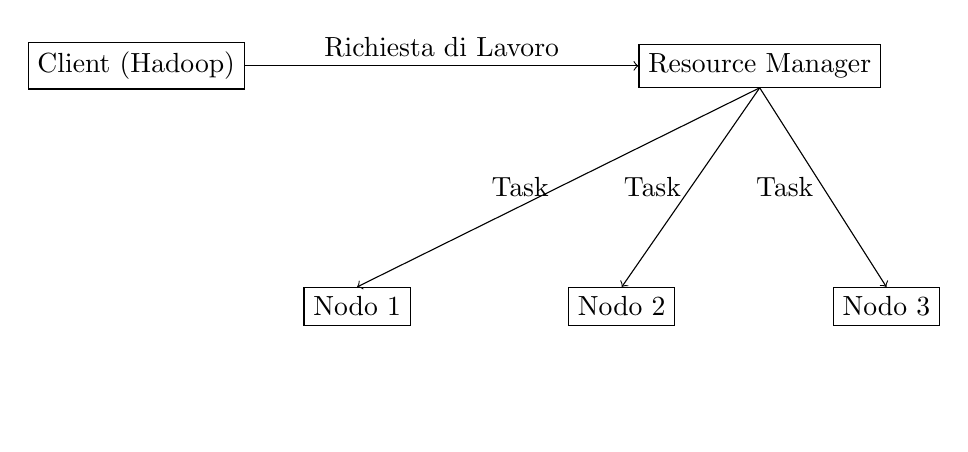
\begin{tikzpicture}

    % Client
    \node [draw, rectangle] (client) {Client (Hadoop)};
    \node [below=4cm of client] (dummy) {}; % Dummy node for spacing

    % Resource Manager
    \node [draw, rectangle, right=5cm of client] (rm) {Resource Manager};
    \node [below=2cm of rm] (dummy2) {}; % Dummy node for spacing

    % Nodi
    \node [draw, rectangle, above right=1cm and 2cm of dummy] (node1) {Nodo 1};
    \node [draw, rectangle, right=2cm of node1] (node2) {Nodo 2};
    \node [draw, rectangle, right=2cm of node2] (node3) {Nodo 3};

    % Freccia da Client a Resource Manager
    \draw[->] (client.east) -- (rm.west) node[midway, above] {Richiesta di Lavoro};

    % Freccia da Resource Manager a Nodi
    \draw[->] (rm.south) -- (node1.north) node[midway, left] {Task};
    \draw[->] (rm.south) -- (node2.north) node[midway, left] {Task};
    \draw[->] (rm.south) -- (node3.north) node[midway, left] {Task};

\end{tikzpicture}

\newpage

